%
% algorithms
% @author Tobias Weber <tweber@ill.fr>
% @date aug-2021
% @license see 'LICENSE' file
%

\chapter{Basic Concepts, Algorithms and Data Structures}
\label{ch:algos}
The  path-finding algorithm and implementation that will be presented in the following chapters
employ several different concepts, data structures and methods.
Among these concepts are the Voronoi diagram (section \ref{sec:voro}),
graph data structures and algorithms on them (section \ref{sec:graphs}),
as well as spatial index trees (section \ref{sec:indextrees}).
In this chapter, these basic building blocks are reviewed in a general manner.



\section{Voronoi diagrams}
\label{sec:voro}
As we will see in the next chapter, a concept that will play a central role for the path-finding 
algorithm of this work is the Voronoi diagram.
A good review of Voronoi diagrams is given in Ref. \cite[Ch. 7, pp. 147-171]{Berg2008} 
and in \cite[Ch. 5, pp. 209f]{FUH_geo2020}, which we follow in this chapter.

Starting with some basic definitions, a \textit{Voronoi diagram} is a set of 
\textit{bisectors}, $B\left(\underline{x},\, \underline{y}\right)$, separating \textit{Voronoi regions}.
A Voronoi region names the set of points $\underline{x}$ in a vector space $V$ that are closest to 
a given site $\underline{s}$ under a given metric $\left\Vert \cdot \right\Vert$, which measures distances in $V$.
The site can either be isolated vertices, lines or any other finite object.
Formally, the bisector between two sites $\underline{s}_1$ and $\underline{s}_2$ is, 
generalising from \cite[p. 140]{Icking2001},
\begin{equation}
	B\left(\underline{s}_1,\, \underline{s}_2\right)\ =\ \left\{ \underline{x} \in V \ |\ 
		\left\Vert \underline{x} - \underline{s}_1 \right\Vert = \left\Vert \underline{x} - \underline{s}_2 \right\Vert \right\}.
	\label{eq:bisector}
\end{equation}
Even though this definition of Voronoi diagrams does not restrict the vector space to the $\mathbb{R}^n$ 
and the underlying metric to the usual Euclidian one, 
\begin{equation}
	\left\Vert \underline{x} \right\Vert_2 \ =\ \sqrt{\left<x | x \right>},
\end{equation}
they are nevertheless implied in the rest of this work if nothing else is specified.
Specifically, we thus set $V = \mathbb{R}^2$ and $\left\Vert \cdot \right\Vert = \left\Vert \cdot \right\Vert_2$. 
Please refer to Ref. \cite{Icking2001} for other metrics and to Ref. \cite{Boissonnat2006} for further 
generalisations of the concept of Voronoi diagrams.



\subsection{Voronoi diagrams for vertex sites}
The simplest case to consider is the Voronoi diagram where the sites are vertices, 
the vector space is the $\mathbb{R}^n$ and the metric Euclidian. This case is called the 
\textit{affine Voronoi diagram} in the work by Boissonnat \textit{et al.},
its bisectors consist of $n-1$-dimensional hyperplanes \cite[pp. 72-81]{Boissonnat2006}.
Specifically for $\mathbb{R}^2$, the bisectors are either line segments or infinite lines, 
depending on the open or closed nature of the corresponding Voronoi region.
An example of two or several vertex sites and their bisectors is shown in Fig. \ref{fig:vertex_voro}.

\begin{figure}[htb]
	\begin{minipage}{1 \textwidth}
		\begin{center}
			\includegraphics[width = 0.35 \textwidth]{figures/vertex_voro}
		\end{center}
		\vspace{0.5cm}
		\begin{center}
			\includegraphics[width = 0.7 \textwidth]{figures/vertex_voro2}
		\end{center}
	\end{minipage}
	\caption[Voronoi diagrams for vertices.]{
		Top panel: Voronoi diagram for two vertex sites, $s_1$ and $s_2$. 
			The bisector, $B\left(s_1, s_2\right)$, separates $\mathbb{R}^2$ 
			into two open Voronoi regions forming half-planes.
		Bottom panel: Voronoi diagram for ten vertex sites, $s_1,\, s_2,\, ...,\, s_{10}$.
		The black lines are the bisectors of the Voronoi regions, where the solid lines are of finite size
		and delimit closed Voronoi regions. The dashed lines are of infinite length and delimit open Voronoi regions.
		The figure has been calculated using the test program that will be described in chapter \ref{sec:tests_hull}.
		\label{fig:vertex_voro}}
\end{figure}


\paragraph{Physical application: Brillouin zones}
Vertex-site Voronoi diagrams are ubiquitous in solid-state physics and all its connected disciplines
like neutron scattering, magnetism, etc., although they are not called so in these fields.
In physics, one usually thinks in terms of the reciprocal (dual, Fourier) space of a crystal lattice, as discussed
in chapter \ref{ch:xtal}. Due to the periodic nature of the crystal and its reciprocal space, one can define a smallest
cell around the vertex sites in reciprocal space (here called ``Bragg peaks'', as discussed before) for which all physics is 
the same, the so-called \textit{first Brillouin zone} of the reciprocal lattice \cite[pp. 63-64]{Gross2012}. 
The definition of the first Brillouin zone corresponds to that of the Voronoi region of the Bragg peaks.
The crystal and its reciprocal lattice are assumed to be infinite. This is a good approximation as one usually
considers physics in the \AA{}ngstr\"om scale ($10^{-10}\,\mathrm{m}$), while the crystals used in neutron scattering usually have volumes on the
$cm^3$ scale. Having an infinite lattice has the effect that the Voronoi diagram does not possess any open, infinite regions.
As the crystal is regular and periodic, only one shape of Voronoi region exists, which repeats to fill the
entire reciprocal space without gaps.
Typical examples of Brillouin zone shapes for cubic crystals and two-dimensional cuts through them 
are shown in Fig. \ref{fig:cubic_bzs}.

\begin{figure}[h]
	\begin{center}
		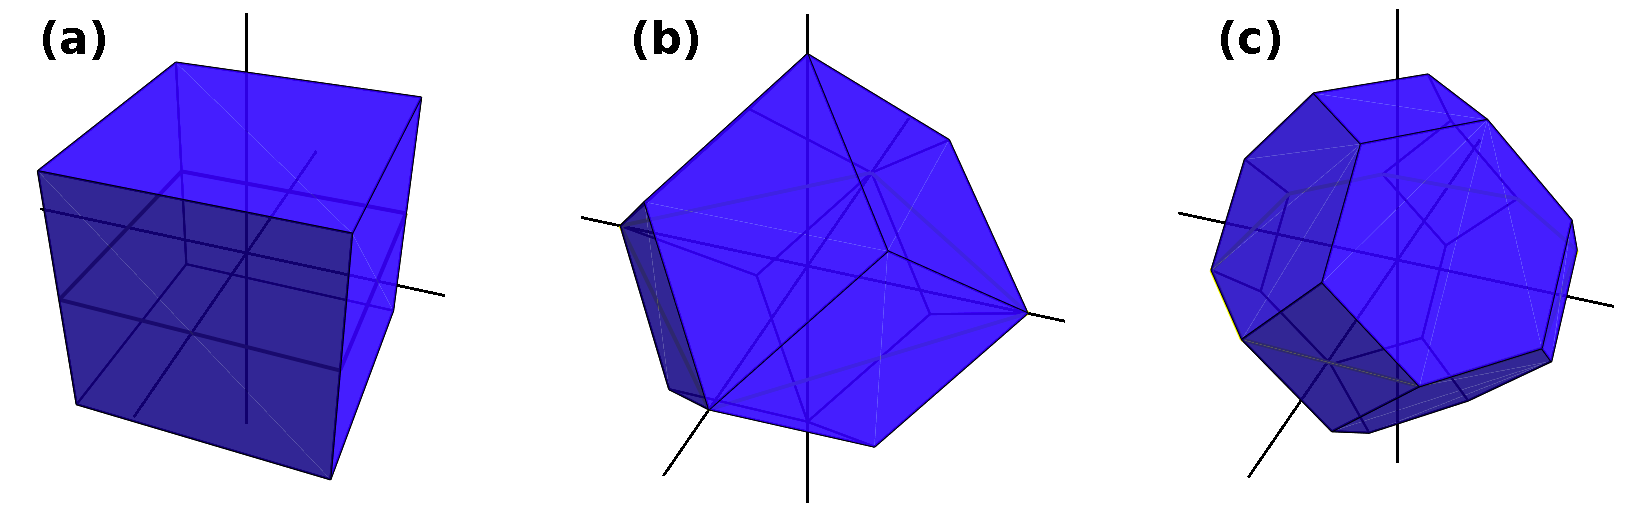
\includegraphics[width = 0.95 \textwidth]{figures/bz}

		\vspace{0.5cm}
		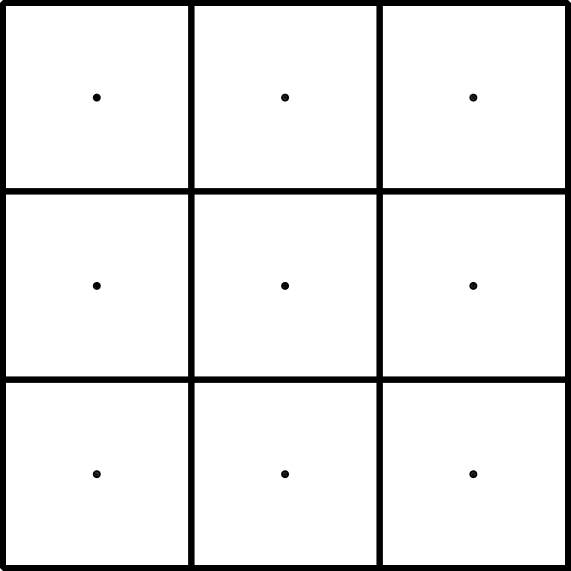
\includegraphics[width = 0.2 \textwidth]{figures/sc}
		\hspace{2.2cm}
		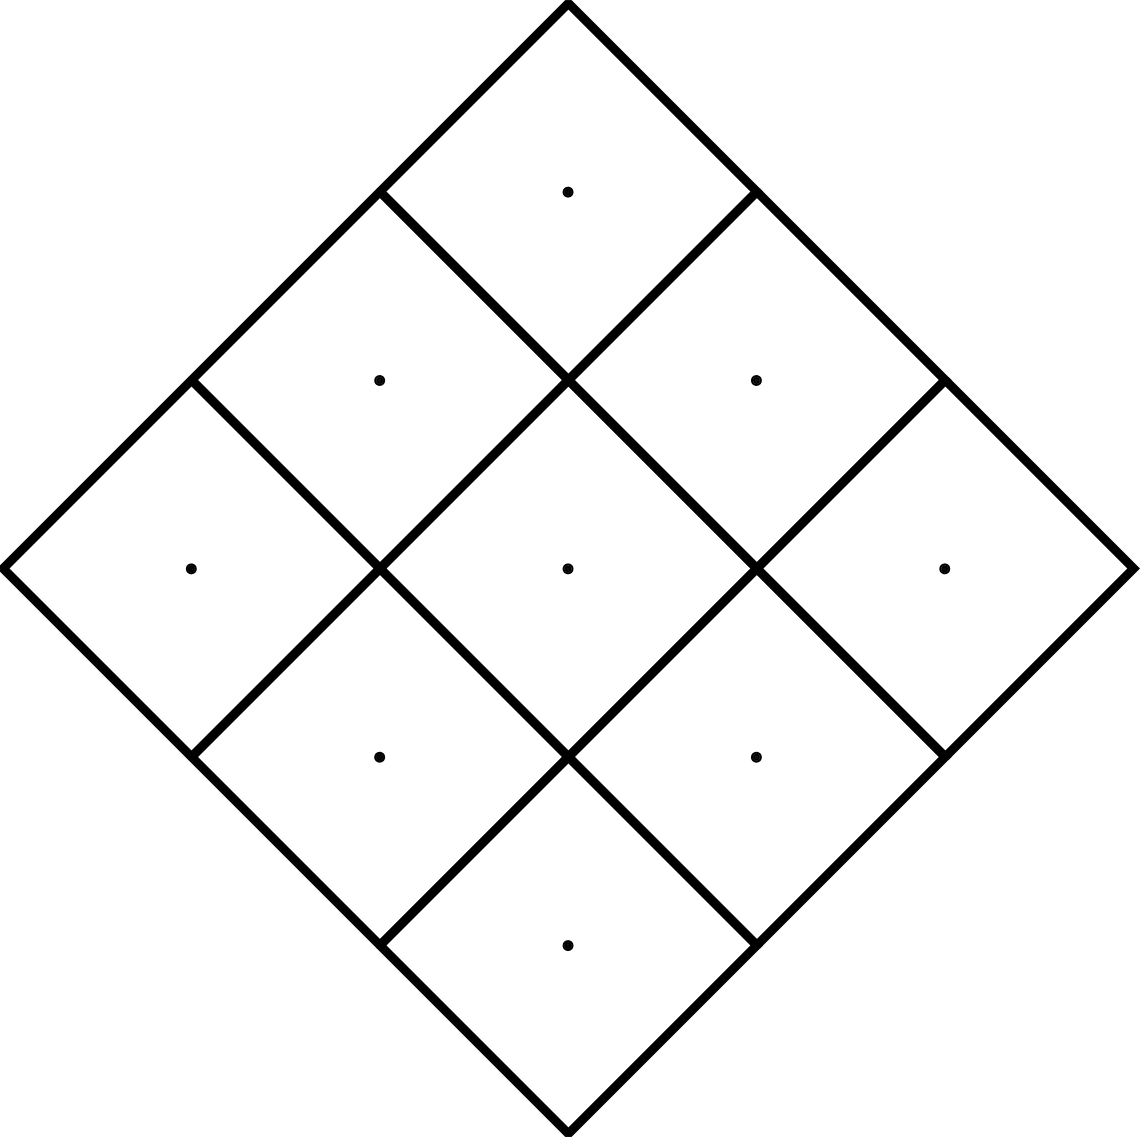
\includegraphics[width = 0.2 \textwidth]{figures/bcc}
		\hspace{2.2cm}
		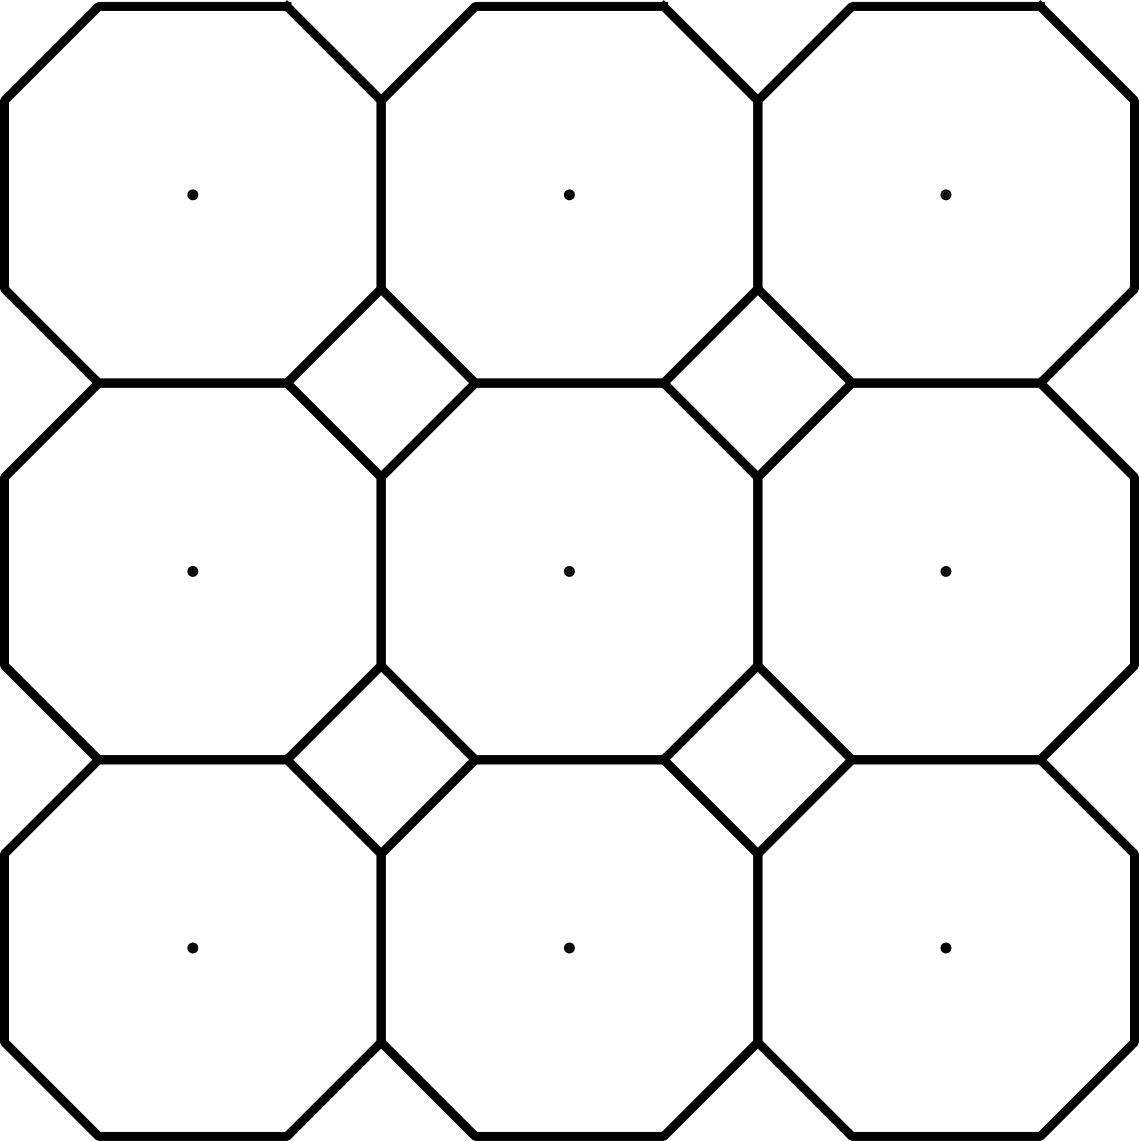
\includegraphics[width = 0.2 \textwidth]{figures/fcc}
	\end{center}
	\caption[Brillouin zones.]{
		First Brillouin zone for
			(a) a simple cubic,
			(b) a body-centred cubic, and
			(c) a face-centred cubic crystal lattice.
		In the top panels, 3-d views of only the bisectors are shown.
		In the bottom panels, 2-d cuts through the horizontal plane show the Brillouin zones 
		completely filling the space. The vertex sites (Bragg peaks) are shown as small dots.
		Such 2-d views are typically used for experiments at triple-axis spectrometers.
		The apparent gaps in in the 2-d cut of panel (c) come from Brillouin zones which are 
		above or below the cutting plane.
		Calculated using the \textit{Takin} software \cite{Takin2021, Takin2017, Takin2016}.
		\label{fig:cubic_bzs}}
\end{figure}



\subsection{Voronoi diagrams for line segment sites}
\label{sec:voro_ls}
Voronoi diagrams over the vector space $\mathbb{R}^n$ with either a non-Euclidian metric or sites that
are not point-shaped are called non-affine and possess curved bisectors \cite[p. 72]{Boissonnat2006}.
We now look at the special case of Voronoi diagrams over the $\mathbb{R}^2$ constructed from line segments.
A description of this case can be found in \cite[Ch. 7.3, pp. 160-163]{Berg2008} and in 
\cite[pp. 242-247]{FUH_geo2020}, whose descriptions we follow in this section.

For this case, the Voronoi region of a line $l_i$ consists of all points in $\mathbb{R}^2$ that 
are closest to $l_i$. The bisector is the boundary between the Voronoi regions of two line segments 
$l_i$ and $l_j$, $i \neq j$,
and is the curve of equal distance between the two line segments $l_i$ and $l_j$.
Its shape is either linear or quadratic, where, in the linear case, the bisector curve can also be either
finite or infinite \cite[pp. 243-244]{FUH_geo2020}.

A linear bisector is obtained for the distance calculated between two line segment endpoints or between two inner 
points on the line segments which are not the endpoints.
This can easily be seen, because, (a) in the case of two endpoints, the middle perpendicular line between these 
two points is equidistant to them; and (b) in the case of two line segments, the angular bisector of the two lines is
equidistant to them \cite[pp. 243-244]{FUH_geo2020}.
On the other hand, the bisector curve segment follows a parabolic shape if the distance is calculated 
between a line segment endpoint and one inner point of the other segment. This is the same as the bisector between
a point and a line and its parabolic shape is proven in \cite[pp. 260-261]{FUH_geo2020}.
An example of two or several line segment sites and their bisectors is shown in Fig. \ref{fig:linesegs_voro}.

\begin{figure}[H]
	\begin{minipage}{1 \textwidth}
		\begin{center}
			\includegraphics[width = 0.7 \textwidth]{figures/linesegs}
		\end{center}
		\vspace{0.5cm}
	\end{minipage}
	\begin{minipage}{1 \textwidth}
		\vspace{0.25cm}
		\begin{center}
			\includegraphics[width = 0.95 \textwidth]{figures/linesegs2}
		\end{center}
	\end{minipage}
	\caption[Voronoi diagrams for line segments.]{
		Top panel: Voronoi regions for two line segments, $l_1$ and $l_2$.
		Bottom panel: Voronoi regions for five line segments, $l_1,\, l_2,\, ...,\, l_5$.
		The line segments and their endpoints are marked in blue. The small red points represent the Voronoi vertices.
		The black lines are the bisectors of the Voronoi regions, where the solid lines delimit finite and the dashed lines
		infinite regions. Helper lines are marked in red. The figure has been calculated using the line segments
		test program which will be described in chapter \ref{sec:tests_linesegs}. The program uses 
		the \textit{Boost.Polygon} library \cite{web_boost_polygon_voronoi}.
		\label{fig:linesegs_voro}}
\end{figure}




\subsection{Voronoi diagrams for curves}
\label{sec:voro_median}
A generalisation of Voronoi diagrams for curves, or, more generally, curved hypersurfaces are the so-called 
\textit{medial axes} \cite{wiki_medial}, that are comprehensively described in 
Refs. \cite[pp. 109-114]{Boissonnat2006} and \cite[pp. 244-252]{Cazals2006}, both of which we follow here.

Our definition of the bisector from Eq. \ref{eq:bisector} is almost general enough to also be valid for medial axes,
but in difference to Eq. \ref{eq:bisector} we now have to consider sites that are not restricted to discrete points or 
objects anymore, but instead are the infinite set of points forming a curve or surface $S$.
Bisectors in the sense of medial axes are now defined in the most general form as the set of points
embedded in a given vector space $V$ without the sites themselves which are closest to two (or more) 
sites under a given metric \cite[p. 244]{Cazals2006}.

For the cases considered in this work, the medial axes coincide with the so-called \textit{topological 1-skeletons} 
\cite{wiki_skeleton, wiki_nskeleton, wiki_medial2} \cite[p. 169]{Berg2008}, which comprise the curves obtained from the centre positions of all possible maximal 
spheres on the hypersurface $S$; this is explained in detail and with more mathematical rigor in the work by 
Cazals and Giesen \cite[pp. 246f]{Cazals2006}.
As we will be interested in these skeletons for the mesh-building step of our path-finding algorithm in the next
chapter, it is important to note that they are notoriously difficult to calculate in a mathematically closed form.
In this work, we will follow the alternate route laid out by Boissonat \textit{et al.}, where the skeleton is 
not calculated directly, but approximated by quantising the surface boundary of $S$ on a grid and calculating 
the Voronoi diagrams for these now finite sets of sites instead of the continuous surface \cite[pp. 109-110]{Boissonnat2006}.
Specifically for $\mathbb{R}^2$, we approximate the boundaries of the site surfaces (here then: curves) 
using line segments and calculate their line segment Voronoi diagram from section \ref{sec:voro_ls} to get 
approximations of the skeletons to the site curves.




\subsection{Software libraries}
A stable and efficient C/C++ library for calculating Voronoi diagram in $\mathbb{R}^n$ is the popular and very 
high-quality \textit{QHull} library by C. B. Barber \cite{web_qhull}. While it does only calculate 
the Voronoi diagrams for vertices, and not for line segments, it is also capable of calculation the Delaunay
triangulation and -- as the name implies -- convex hull of the sites.
The \textit{OpenCV} library \cite{web_opencv} also features a module for calculating Voronoi diagrams
(and the dual Delaunay triangulation), but is also restricted to vertex sites and to two dimensions.

Several libraries for calculating the line segment Voronoi diagrams in $\mathbb{R}^2$ exist, noteworthy 
are \textit{VRONI} by M. Held \cite{Held2001}, \textit{OpenVoronoi} by A. E. Wallin \cite{web_openvoronoi}, \textit{VoroLS} 
by W. Schumann \cite{DiplomaSchumann}, as well as the Voronoi calculator \cite{web_boost_polygon_voronoi} 
by A. Sydorchukof, which is part of the \textit{Boost.Polygon}  \cite{web_boost_polygon, Simonson2009} 
C++ library.
A further noteworthy library, which is capable of caluclating 2D Voronoi diagrams and Delaunay triangulations
for both vertex and line segment sites is the \textit{2D Segment Delaunay Graphs} library by M. Karavelas \cite{web_2dsegdel, Karavelas2004, Karavelas2006} 
which is part of the \textit{CGAL} \cite{web_cgal} software package.
The first three libraries are not feasible for the present project, though: 
\begin{itemize}
	\item \textit{VRONI} \cite{Held2001} is reported in a paper, but is neither freely available 
		nor under a suitable open-source license.
	\item The opposite is true for \textit{OpenVoronoi} \cite{web_openvoronoi}: 
		It is available under an open-source license, but our first tests deemed it too unstable 
		for use in a production-quality software. 
		The source code for our tests can be found in the function \lstinline[language=C++]|geo::calc_voro_ovd()|, 
		which resides in file \lstinline|./src/libs/voronoi_lines.h| of the accompanying code archive. 
		The source code for the test tool itself is located in: \lstinline|./src/tools/lines.cpp|.
	\item \textit{VoroLS} \cite{DiplomaSchumann} is stable and does even handle intersecting lines, but is a \textit{Java}
		software, not a library, and is not under an open-source license.
	\item All requirements were met by \textit{Boost.Polygon} \cite{web_boost_polygon}, though, and we will use 
		this library for the calculations of the present work.
		\textit{Boost.Polygon} uses Fortune's sweep algorithm \cite{Fortune1987} to construct
		the Voronoi diagram, which has an upper bound in complexity of $\mathcal{O}\left( n \log_2 n \right)$ in time
		and $\mathcal{O}\left( n \right)$ in storage space for $n$ line segments \cite[p. 168]{Fortune1987}.
		The library is internally based on integers coordinates for optimal performance \cite{web_boost_polygon}.
		The reliance on integer coordinate representation is also responsible for \textit{Boost.Polygon}'s 
		inability to handle intersecting lines, because the intersection point may be at a non-integer coordinate. 
		Intersecting lines need to be carefully filtered out before calculation, because they can unfortunately cause the 
		\textit{Boost.Polygon} library to either crash, hang, or yield wrong bisectors.
		An advantage of using integers is that we can create polygonal objects out of line segments and calculate
		their Voronoi diagrams without having to define an epsilon environment for coinciding vertices.
	\item The \textit{CGAL / 2D Segment Delaunay Graphs} library \cite{web_2dsegdel, Karavelas2004, Karavelas2006}
		also fulfills all requirements with respect to its open-source licensing model and capabilities,
		and we will use it as alternate calculation backend for the software of this work.
		It is capable of calculating line segment Voronoi diagrams even for intersecting line segments.
		As is discussed by Boissonat \textit{et al.}, \textit{2D Segment Delaunay Graphs} uses an incremental
		algorithm \cite[pp. 114-115]{Boissonnat2006}, which has a worst-case time complexity of only
		$\mathcal{O}\left( n \log_2^2 n \right)$ for live-inserting $n$ line segments \cite[p. 104]{Boissonnat2006}, 
		but can also achieve $\mathcal{O}\left( n \log_2 n \right)$ when inserting the line segments in randomised 
		order \cite[p. 105]{Boissonnat2006}.
\end{itemize}


\paragraph{Performance comparison}
Figure \ref{fig:voro_performance} shows a performance comparison between the \textit{Boost.Polygon} and
the \textit{CGAL / 2D Segment Delaunay Graphs} libraries.
The curves depict the times needed to calculate the Voronoi diagrams for random non-intersecting line segments
using a \textit{AMD Ryzen 7 2700} CPU.
Several runs were performed for an increasing number of line segments and the same random line segments were
used as input for both libraries per run.
It is interesting to note that both libraries exhibit virtually the same performance, meaning they are both
well-optimised.
A second set of runs was performed, comparing the run times of binaries generated by two different C++ compilers,
\textit{GCC} \cite{web_gcc} (version 10.3.1) and \textit{Clang} \cite{web_clang} (version 11.0.0).
It can be observed that the \textit{GCC} compiler clearly outperforms \textit{Clang}.
Such a significant influence of the compiler is most likely due to both libraries being generic template meta
programs, which gives the compilers' optimisation stages some play.
Note that the random lines were different between the two compiler runs, but this cannot explain the better
performance of the executable generated by \textit{GCC}, because it is improbable that line segments that
are easier for Voronoi diagram calculation had been generated for every single run of the \textit{GCC} dataset.


\begin{figure}[htb]
	\begin{center}
		\includegraphics[width = 0.55 \textwidth, trim=0.5cm 0.2cm 0.5cm 0.75cm, clip]{figures/voronoi_performance}
	\end{center}
	\caption[Voronoi calculation performance.]{
		Comparison of the times needed to calculate the line segment Voronoi diagrams for an increasing
		number of random line segments using the \textit{Boost.Polygon} (labelled ``Boost'') \cite{web_boost_polygon}
		and the \textit{CGAL / 2D Segment Delaunay Graphs} (``CGAL'') \cite{web_2dsegdel} libraries.
		\label{fig:voro_performance}}
\end{figure}



\section{Graphs}
\label{sec:graphs}
Another crucial concept for path-finding on a mesh of nodes is the graph.
A good review of graph theory can be found in Ref. \cite{FUH_algo_graphs_2021},
which we will follow in this section.

A graph is a tuple $G = \left(V, E\right)$ of a set of vertices $V$ and edges $E \subseteq V \times V$ 
connecting the vertices. For the present case, we only consider directed and weighted graphs 
\cite[pp. 1-3]{FUH_algo_graphs_2021}.
\textit{Directed} means that the existence of an edge $e = \left(v_1, v_2\right)$ connecting vertices 
$v_1 \in V$ and $v_2 \in V$ does not imply the existence of the reverse connection $e'= \left(v_2, v_1\right)$
from $v_2$ to $v_1$. That would only be the case in an undirected graph.
\textit{Weighted} means that a weight function $w: E \rightarrow \mathbb{R}$ exists which maps each 
edge $e \in E$ to a weight factor $w\left(e\right) \in \mathbb{R}$ quantifying that edge. 
For example, the weight factors could be distances for a graph whose vertices also correspond to Cartesian coordinates.
Another restriction that will be used in this work is the exclusion of loops in the graph, i.e.
no edges $e = \left(v, v\right)$ connecting a vertex $v \in V$ to itself will be allowed.
Finally, we define a path in the graph as a tuple of $n$ vertices $p = \left(v_1, v_2, ..., v_n\right)$
where subsequent vertices $v_i$ and $v_{i+1}$, $i \in \left[1, n\right]$, are connected by an edge and 
where each vertex in the tuple is unique, i.e. $v_i \neq v_j$ for $i \neq j$.
Specifically, this signifies that there are no loops and no vertex is visited multiple times upon 
traversal of the path.
An example for a directed and weighted graph is shown in Fig. \ref{fig:example_graph}.
This example graph will also serve for the algorithm demonstrations in the following.

\begin{figure}[h]
	\begin{center}
		\includegraphics[width = 0.9 \textwidth, trim=1cm 1cm 1cm 1cm, clip]{figures/example_graph}
	\end{center}
	\caption[Example graph.]{
		Example of a directed, weighted graph containing five vertices, $v_1$, $v_2$, ..., $v_5$.
		The figure has been drawn using the \textit{Dot} tool from the \textit{Graphviz} software \cite{Ellson2003}.
		\label{fig:example_graph}}
\end{figure}


\paragraph{Data structures}
There are two common data structures to store graphs, the adjacency matrix and the adjacency list, which are
both discussed in general and in terms of complexity in Ref. \cite[pp. 3-5]{FUH_algo_graphs_2021}.
The adjacency matrix for a graph with $n$ vertices is an $n \times n$ matrix that stores the 
weights $w\left(e_{ij}\right)$ for edge $e_{ij}$ between vertices $v_i$ and $v_j$ in its elements,
where either $0$ or a special \textit{null} symbol means that the corresponding edge does not exist.
The adjacency list for a graph with $n$ vertices is an array with $n$ elements $l_i$ which point 
to the head of a (doubly) linked list whose entries contain pointers to all the vertices $v_j$ that are reachable 
from vertex $v_i$ along with the weight factors for edge $e_{ij}$.
Table \ref{tab:example_graph_structure} shows an example for an adjacency matrix and an adjacency list.

\begin{table}[h]
	\centering
	\begin{tabular}{|c|ccccc|}
			\hline
			      & $v_1$ & $v_2$ & $v_3$ & $v_4$ & $v_5$ \tabularnewline
			\hline
			$v_1$ &  null &     1 &  null &     9 &    10 \tabularnewline
			$v_2$ &  null &  null &     3 &     7 &  null \tabularnewline
			$v_3$ &    10 &  null &  null &     1 &     2 \tabularnewline
			$v_4$ &  null &     1 &  null &  null &     2 \tabularnewline
			$v_5$ &  null &  null &  null &  null &  null \tabularnewline
			\hline
	\end{tabular}
	\hspace{1cm}
	\begin{tabular}{|c|c|ccccc|}
			\cline{1-1} \cline{3-7}
			$v_1$ &  $\rightarrow$ &  $v_2\, [1]$ &  $\leftrightarrow$ &  $v_4\, [9]$ &  $\leftrightarrow$  & $v_5\, [10]$ \tabularnewline
			\cline{1-1} \cline{3-7}
			$v_2$ &  $\rightarrow$ &  $v_3\, [3]$ &  $\leftrightarrow$ &  $v_4\, [7]$ &   &  \tabularnewline
			\cline{1-1} \cline{3-7}
			$v_3$ &  $\rightarrow$ &  $v_1\, [10]$ &  $\leftrightarrow$ &  $v_4\, [1]$ &  $\leftrightarrow$  & $v_5\, [2]$ \tabularnewline
			\cline{1-1} \cline{3-7}
			$v_4$ &  $\rightarrow$ &  $v_2\, [1]$ & $\leftrightarrow$  &  $v_5\, [2]$ &   &  \tabularnewline
			\cline{1-1} \cline{3-7}
			$v_5$ &  $\rightarrow$ & null &   &   &   &  \tabularnewline
			\cline{1-1} \cline{3-7}
	\end{tabular}
	\caption[Adjacency matrix and list.]{
		Adjacency matrix (left) and adjacency list (right) for the example graph shown in Fig. \ref{fig:example_graph}.
		For the adjacency matrix, the weight factors directly form the entries, whereas for the adjacency list, 
		the weight factors are stored alongside the vertex entries and are here shown in square brackets.
		These tables follow the design of Ref. \cite[pp. 4, table 4.1]{FUH_algo_graphs_2021}.}
	\label{tab:example_graph_structure}
\end{table}



\subsection{Shortest path and Dijkstra's algorithm}
\label{sec:dijkstra}
\paragraph{Shortest path}
The shortest path in a graph is the path between two vertices which minimises the sum of the weights
of all edges that are traversed along the way.
Two general classes of algorithms for finding the shortest path in a graph exist.
The first class of algorithms solves the so-called \textit{single source shortest path (SSSP)} problem,
which calculates the shortest paths from one source vertex to all other vertices \cite[pp. 273-297]{Erickson2019}.
The second class of algorithms solves the \textit{all pairs shortest path (APSP)} problem, which calculates
all possible pairs of shortest paths between any two vertices in the graph \cite[pp. 309-320]{Erickson2019}.
Noteworthy representatives of these two classes are the Bellman-Ford \cite[pp. 11-14]{FUH_algo_graphs_2021} 
and the Dijkstra algorithm \cite[pp. 14-18]{FUH_algo_graphs_2021} for SSSP, 
as well as the Johnson \cite[pp. 19-21]{FUH_algo_graphs_2021} 
and the Floyd-Warshall algorithm \cite[pp. 21-24]{FUH_algo_graphs_2021} for APSP.

For the case presented in the following chapters we are interested in calculating a single path between 
a source and target point and will thus need to solve an SSSP problem.
To that end we choose Dijkstra's algorithm, because in the best case it can be implemented 
in $\mathcal{O}\left( n_e \log_2 n_v \right)$ time and $\mathcal{O}\left( n_v \right)$ space 
complexity when using a heap as internal data structure \cite[pp. 17-18]{FUH_algo_graphs_2021}, 
where $n_v$ is the number of vertices in the graph, and $n_e$ the number of edges.
The Bellman-Ford algorithm would be less efficient, with time and storage complexities of 
$\mathcal{O}\left( n_v n_e \right)$ and $\mathcal{O}\left( n_v \right)$, respectively 
\cite[pp. 13]{FUH_algo_graphs_2021}.

\paragraph{Dijkstra's algorithm}
Following the pseudo-code description in Ref. \cite[p. 17]{FUH_algo_graphs_2021}, Dijkstra's algorithm
works by inserting all vertices of the graph into a priority search queue, where they are sorted according 
to distances values to the start vertex that are to be determined and which are initially set to $0$ for
the start vertex and to infinity for all other vertices.
As long as the priority queue is not empty, its top vertex, i.e. the one with the lowest distance value, 
$v_i$, is removed from it. 
It is tested for each of $v_i$'s outgoing edges, $e_{ij}$, if the path length from the start vertex to 
vertex $v_j$ (saved as the distance value for $v_j$) becomes smaller when going over vertex $v_i$ (determined
as the distance value for $v_i$ plus the weight of the edge $e_{ij}$). 
If so, the distance value for $v_j$ is set to this shorter path length and $v_i$ is remembered as the
predecessor of $v_j$ along the path.
In total, Dijkstra's algorithm is at its core a breath-first search of a graph, where the next neighbour 
vertex to visit is chosen by the lowest weight factor of the connecting edges.
As discussed before, the priority search queue has to use a heap as its internal data structure for
optimal run time.

It should be noted that while this is the textbook example of Dijkstra's algorithm, J. Erickson describes
a slightly modified version which is more general in its support of negative edge weights and which is not
less efficient than the standard version \cite[pp. 284-288]{Erickson2019}:
This modified version does not directly initialise the priority search queue with all vertices beforehand, 
but only with the start vertex (using, as before, a distance of $0$ to itself).
It inserts the neighbour vertices $v_j$ (as defined above) only if they are discovered to lead to a shorter 
path in the iteration of all neighbours of the current top vertex in the queue, $v_i$. Full pseudo-code 
for that can be found in Ref. \cite[p. 285]{Erickson2019}.

\paragraph{Example}
The two variants of Dijkstra's algorithm are best demonstrated using an example.
In table \ref{tab:example_dijk} we show each step of the algorithm by finding the shortest
paths from start point $v_1$ of the graph in Fig. \ref{fig:example_graph}.
From the final results, a shortest path can be constructed by traversing the predecessors in
reverse. For instance, for the shortest path from $v_1$ to $v_5$ we look at the predecessor
of $v_5$, which is $v_3$. Next, the predecessor of $v_3$ is $v_2$ and that of $v_2$ is $v_1$.
The shortest path is thus $v_1$, $v_2$, $v_3$, $v_5$.

\begin{table}[h]
	\begin{minipage}[t]{0.45 \textwidth}
	Dijkstra's algorithm \cite[p. 17]{FUH_algo_graphs_2021} run:
	\begin{itemize}
	\item Initialisation.
	
	\begin{tabular}{|c|ccccc|}
			\hline
			     Heap & $v_1$ & $v_2$ & $v_3$ & $v_4$ & $v_5$ \tabularnewline
			\hline
			Distances &  $0$  &  $\infty$ &  $\infty$ &     $\infty$ &    $\infty$ \tabularnewline
			\hline
	\end{tabular}\\
	\begin{tabular}{|c|ccccc|}
			\hline
			     Vertices & $v_1$ & $v_2$ & $v_3$ & $v_4$ & $v_5$ \tabularnewline
			\hline
			Predecessors &  -  &  - &  - &     - &    - \tabularnewline
			\hline
	\end{tabular}
	

	\item Iteration 1: Outgoing edges from $v_1$ to $v_2$, $v_4$, and $v_5$
		all lead to shorter paths.
	
	\begin{tabular}{|c|cccc|}
			\hline
			     Heap & $v_2$ & $v_4$ & $v_3$ & $v_5$ \tabularnewline
			\hline
			Distances &  $1$  &  $9$ &  $\infty$ &     $10$  \tabularnewline
			\hline
	\end{tabular}\\
	\begin{tabular}{|c|ccccc|}
			\hline
			     Vertices & $v_1$ & $v_2$ & $v_3$ & $v_4$ & $v_5$ \tabularnewline
			\hline
			Predecessors &  -  &  $v_1$ &  - &     $v_1$ &    $v_1$ \tabularnewline
			\hline
	\end{tabular}


	\item Iteration 2: Outgoing edges from $v_2$ to $v_3$ and $v_4$
		both lead to shorter paths.
	
	\begin{tabular}{|c|ccc|}
			\hline
			     Heap & $v_3$ & $v_5$ & $v_4$  \tabularnewline
			\hline
			Distances &  $4$  &  $10$ &  $8$  \tabularnewline
			\hline
	\end{tabular}\\
	\begin{tabular}{|c|ccccc|}
			\hline
			     Vertices & $v_1$ & $v_2$ & $v_3$ & $v_4$ & $v_5$ \tabularnewline
			\hline
			Predecessors &  -  &  $v_1$ &  $v_2$ &     $v_2$ &    $v_1$ \tabularnewline
			\hline
	\end{tabular}


	\item Iteration 3: Outgoing edges from $v_3$ to $v_4$ and $v_5$
		both lead to shorter paths.
	
	\begin{tabular}{|c|cc|}
			\hline
			     Heap & $v_4$ & $v_5$  \tabularnewline
			\hline
			Distances &  $5$  &  $6$   \tabularnewline
			\hline
	\end{tabular}\\
	\begin{tabular}{|c|ccccc|}
			\hline
			     Vertices & $v_1$ & $v_2$ & $v_3$ & $v_4$ & $v_5$ \tabularnewline
			\hline
			Predecessors &  -  &  $v_1$ &  $v_2$ &     $v_3$ &    $v_3$ \tabularnewline
			\hline
	\end{tabular}


	\item Iteration 4: Outgoing edges from $v_4$ to $v_2$ and $v_5$
		do not lead shorter paths.
	
	\begin{tabular}{|c|c|}
			\hline
			     Heap & $v_5$ \tabularnewline
			\hline
			Distance &  $6$   \tabularnewline
			\hline
	\end{tabular}


	\item Finalisation: No outgoing edges from $v_5$.
	
	\begin{tabular}{|c|ccccc|}
			\hline
			     Vertices & $v_1$ & $v_2$ & $v_3$ & $v_4$ & $v_5$ \tabularnewline
			\hline
			Predecessors &  -  &  $v_1$ &  $v_2$ &     $v_3$ &    $v_3$ \tabularnewline
			Distances &  $0$  &  $1$ &  $4$ &     $5$ &    $6$ \tabularnewline
			\hline
	\end{tabular}

	\end{itemize}
	\end{minipage}
	%
	%
	%
	%
	\begin{minipage}[t]{0.45 \textwidth}
	%\footnotesize
	Modified Dijkstra's algorithm \cite[p. 285]{Erickson2019} run:
	\begin{itemize}
	\item Initialisation.
	
	\begin{tabular}{|c|c|}
			\hline
			     Heap & $v_1$ \tabularnewline
			\hline
			Distance &  $0$  \tabularnewline
			\hline
	\end{tabular}\\
	\begin{tabular}{|c|ccccc|}
			\hline
			     Vertices & $v_1$ & $v_2$ & $v_3$ & $v_4$ & $v_5$ \tabularnewline
			\hline
			Predecessors &  -  &  - &  - &     - &    - \tabularnewline
			\hline
	\end{tabular}
	

	\item Iteration 1: Outgoing edges from $v_1$ to $v_2$, $v_4$, and $v_5$
		all lead to shorter paths.
	
	\begin{tabular}{|c|ccc|}
			\hline
			     Heap & $v_2$ & $v_5$ & $v_4$ \tabularnewline
			\hline
			Distances &  $1$  &  $10$ &  $9$ \tabularnewline
			\hline
	\end{tabular}\\
	\begin{tabular}{|c|ccccc|}
			\hline
			     Vertices & $v_1$ & $v_2$ & $v_3$ & $v_4$ & $v_5$ \tabularnewline
			\hline
			Predecessors &  -  &  $v_1$ &  - &     $v_1$ &    $v_1$ \tabularnewline
			\hline
	\end{tabular}


	\item Iteration 2: Outgoing edges from $v_2$ to $v_3$ and $v_4$
		both lead to shorter paths.
	
	\begin{tabular}{|c|ccc|}
			\hline
			     Heap & $v_3$ & $v_5$  &  $v_4$  \tabularnewline
			\hline
			Distances &  $4$  &  $10$  &  $8$  \tabularnewline
			\hline
	\end{tabular}\\
	\begin{tabular}{|c|ccccc|}
			\hline
			     Vertices & $v_1$ & $v_2$ & $v_3$ & $v_4$ & $v_5$ \tabularnewline
			\hline
			Predecessors &  -  &  $v_1$ &  $v_2$ &     $v_2$ &    $v_1$ \tabularnewline
			\hline
	\end{tabular}


	\item Iteration 3: Outgoing edges from $v_3$ to $v_4$ and $v_5$
		both lead to shorter paths.
	
	\begin{tabular}{|c|cc|}
			\hline
			     Heap & $v_4$ & $v_5$  \tabularnewline
			\hline
			Distances &  $5$  &  $6$   \tabularnewline
			\hline
	\end{tabular}\\
	\begin{tabular}{|c|ccccc|}
			\hline
			     Vertices & $v_1$ & $v_2$ & $v_3$ & $v_4$ & $v_5$ \tabularnewline
			\hline
			Predecessors &  -  &  $v_1$ &  $v_2$ &     $v_3$ &    $v_3$ \tabularnewline
			\hline
	\end{tabular}


	\item Iteration 4: No outgoing edges from $v_4$ to $v_2$ and $v_5$
		do not lead to shorter paths.
	
	\begin{tabular}{|c|c|}
			\hline
			     Heap & $v_5$ \tabularnewline
			\hline
			Distance &  $6$   \tabularnewline
			\hline
	\end{tabular}


	\item Finalisation: No outgoing edges from $v_5$.
	
	\begin{tabular}{|c|ccccc|}
			\hline
			     Vertices & $v_1$ & $v_2$ & $v_3$ & $v_4$ & $v_5$ \tabularnewline
			\hline
			Predecessors &  -  &  $v_1$ &  $v_2$ &     $v_3$ &    $v_3$ \tabularnewline
			Distances &  $0$  &  $1$ &  $4$ &     $5$ &    $6$ \tabularnewline
			\hline
	\end{tabular}

	\end{itemize}
	\end{minipage}

	\caption[Example for Dijkstra's algorithm.]{
	Example runs of Dijkstra's algorithm (left column) and its modified version (right column)
	for the graph shown in Fig. \ref{fig:example_graph} and start vertex $v_1$.
	Note that from iteration 2 on, both variants have converged to the same results.}
	\label{tab:example_dijk}
\end{table}




\section{Spatial index trees}
\label{sec:indextrees}
Finding a certain number from a set of $n$ numbers which possess an ordering relation --
alternatively, all numbers that are smaller or greater than a certain number or lie within a range -- 
can be efficiently done in one dimension using a binary search tree.
Several well-known data structures exist, among them the \textit{AVL tree} \cite{wiki_avl} and the 
\textit{Red-black tree} \cite{wiki_redblack}.
Both of them possess a memory complexity linear in the number of elements, $n$, and -- since they 
are balanced with respect to their heights -- dual-logarithmic in time for searching, inserting 
and removing an element \cite{wiki_avl, wiki_redblack}.

In $k$ dimensions, there are several generalisations of search trees, among them the 
\textit{BSP tree} \cite[Ch. 12, pp. 259-281]{Berg2008} and the \textit{k-d tree} \cite[Ch. 5.2, pp. 99-105]{Berg2008}
as examples of multi-dimensional binary search trees, as well as the non-binary
\textit {R tree} \cite{wiki_rtree}.


\paragraph{BSP tree}
Following the definition in Ref. \cite[pp. 261-262]{Berg2008}, a BSP or \textit{binary space partitioning} 
tree divides the $k$ dimensional vector space it operates on into two half-spaces. 
These two half-spaces respectively lie left and right of 
an $k-1$ dimensional splitting hyperplane. The hyperplane is usually chosen so that each of the 
half-spaces contains an equal amount of stored objects (vertices, polygons, etc.). 
The algorithm is next applied recursively to each of the half-spaces, partitioning them in the same
fashion until there is only one object left, yielding a leaf node.


\paragraph{k-d tree}
The $k$-d, or \textit{$k$-dimensional tree} is a special case of the BSP tree where the splitting planes are 
axis-aligned \cite[p. 278]{Berg2008}. 
There is also less freedom to choose them as in the BSP case: In the recursion steps, a split by 
the $x_1 = const.$ plane is followed by the $x_2 = const.$ plane in the next depth level of the tree,
until the $x_k = const.$ plane is reached, after which the choice wraps around to the
$x_1 = const.$ plane. The only freedom is to choose the respective constant offsets of the
plane to have the tree optimally balanced.
A $k$-d tree of $n$ objects can be created with an upper bound in time complexity of 
$\mathcal{O}\left( n \log_2 n \right)$ and has a storage complexity linear in $n$,
its range query time lies in $\mathcal{O}\left( n^{1-1/k} + r \right)$, where $r$ is the number of
objects that are found by the query \cite[p. 105]{Berg2008}.
An example for a k-d tree is shown in Fig. \ref{fig:example_kdtree}.

\begin{figure}[h]
	\begin{center}
		\begin{minipage}{0.4 \textwidth}
			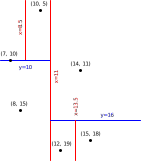
\includegraphics[width = 1 \textwidth]{figures/example_kd_plane}
		\end{minipage}
		\hspace{0.1cm}
		\begin{minipage}{0.58 \textwidth}
			\includegraphics[width = 1 \textwidth, trim=1cm 1cm 1cm 1cm, clip]{figures/example_kd}
		\end{minipage}
	\end{center}
	\caption[Example k-d tree.]{A k-d created from six vertices (left panel) and its graph representation (right panel).
		The vertices are drawn as black circles, the vertical and horizontal splitting planes
		are shown in red and blue, respectively.
		The splitting planes are written out explicitly to emphasise that a
		k-d tree is also a BSP tree (but not necessarily vice versa).
		The graph has been drawn using the \textit{Dot} tool from the \textit{Graphviz} software \cite{Ellson2003}.
		\label{fig:example_kdtree}}
\end{figure}


\paragraph{R tree}
R tree stands for \textit{rectangle tree} and is named for its use of (hyper-)rectangles 
grouping objects \cite{wiki_rtree}.
Each node in the tree has a hyperrectangle assigned to it, which serves as axis-aligned bounding box
for all the objects it contains in its child nodes. 
The tree is not necessarily a binary tree, in fact, the number of children that each node can have is 
a configuration parameter. 
The rectangular bounding boxes for the nodes at the same height may overlap, and the key to efficiency 
in this kind of tree is a good insertion algorithm which minimises such a overlap.
The most prominent of these overlap-minimised data structures is the so-called \textit{R* tree} \cite{wiki_rstartree}.
Fig. \ref{fig:example_rtrees} shows a comparison between a classical R tree and and R* tree for the
same vertex sites. The R trees shows a clearly more pronounced overlap than the R* tree.

\begin{figure}[h]
	\begin{center}
		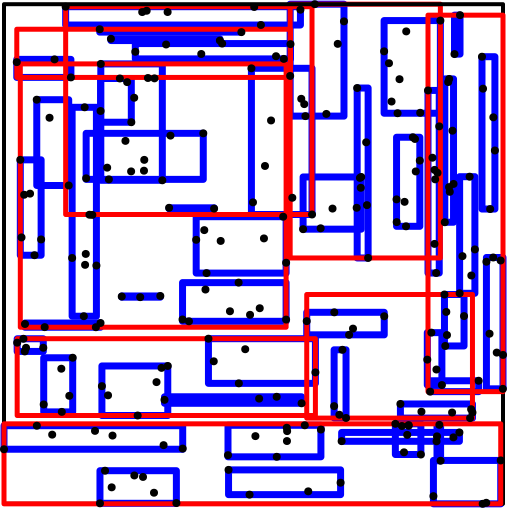
\includegraphics[width = 0.38 \textwidth]{figures/rtree8}
		\hspace{1cm}
		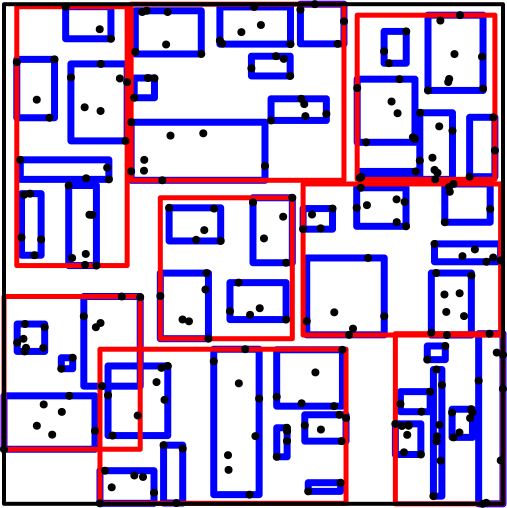
\includegraphics[width = 0.38 \textwidth]{figures/rstartree8}
	\end{center}
	\caption[Example R trees.]{An R tree (left panel) and an R* tree (right panel) for the 
		same 250 random, linearly distributed vertices (back circles). 
		The rectangular bounding boxes at each level of the R trees are marked in different colours, 
		the innermost rectangles are blue, the next level is red, and the outermost level 
		(at the root node) is black.
		The trees were created so that each node has maximally 8 children.
		These panels were calculated using the \lstinline[language=C++]|rtree| class \cite{web_boost_geometry_rtree}
		of the \textit{Boost.Geometry} library \cite{web_boost_geometry}.
		\label{fig:example_rtrees}}
\end{figure}


\subsection{Software libraries}
BSP trees are very popular in the field of computer graphics, and free and open-source implementations are 
readily available \cite{web_bsp_faq}. Unfortunately and surprisingly, the \textit{Boost} C++ libraries \cite{web_boost},
which is the preferred ressource for data types and algorithms in this work, do not feature one. 
Equally surprisingly, the \textit{Qt} libraries do feature a BSP tree implementation, but it is not part of 
their public API, but only used internally in the \lstinline[language=C++]|QGraphicsScene| class \cite{web_QGraphicsScene}.

Open-source k-d tree implementations can be found in \textit{OpenCV} \cite{web_opencv} 
and in \textit{CGAL} \cite{web_cgal}.

A high-quality implementation of R and R* trees as well as the insertion, deletion, and querying algorithms 
operating on them is readily available through the \textit{Boost.Geometry} library \cite{web_boost_geometry, web_boost_geometry_rtree}. As first tests could directly confirm the good performance of \textit{Boost.Geometry}'s,
R and R* tree codes, we will employ them for this work.



\section{Summary}
With the concept of the Voronoi diagram, basic graph theory, and spatial index trees, 
this chapter presented the foundations on which the path-mesh calculation and path-finding
algorithm of this work will be based. The following chapter will review different kinds
of path-finding methods and use parts of these to construct a bespoke method which
is suitable for the angular movement of triple-axis spectrometers.
